\chapter{Process}\label{chap:process}


\section{Development process}

% AGILE

\cite{martin2003agile, highsmith2001agile}

% OPENUP

\cite{balduino2007introduction, kroll2006agility}

% Project Plan Recap

\subsection{Open Source}

\cite{raymond1999cathedral, weber2004success}

% Release early, Release often

\subsection{Version Control}

% GITHUB
\cite{finley2011github}


%%%%%%%%%%%%%%%%%%%%%%%%%%%%
%% Figure: github-project %%
%%%%%%%%%%%%%%%%%%%%%%%%%%%%
\begin{figure}[H]
\centering
    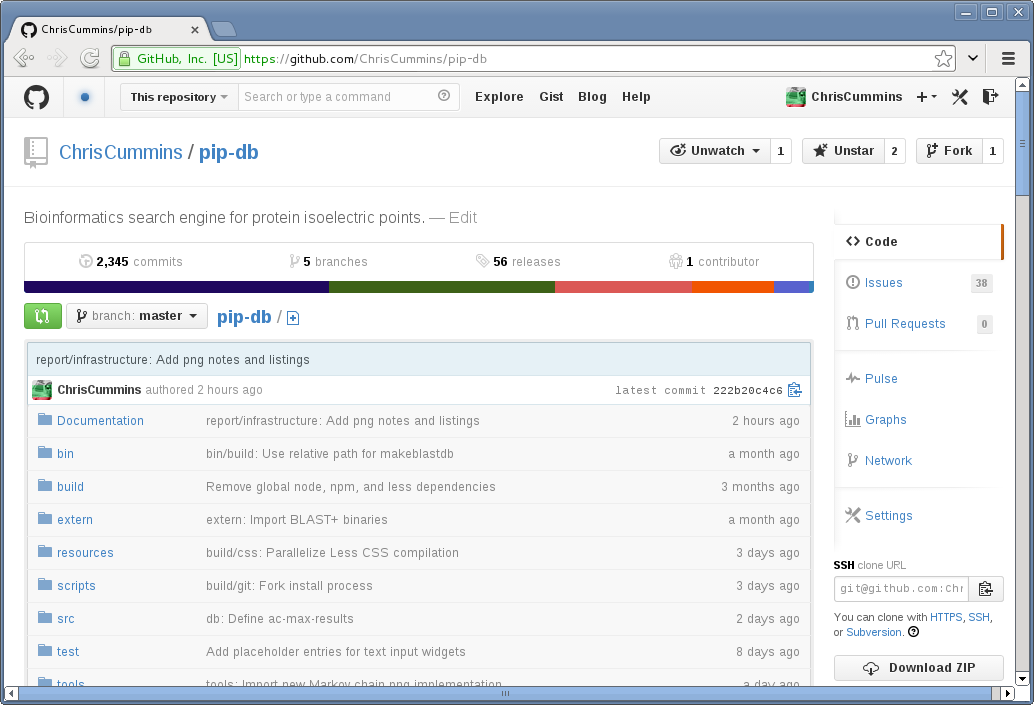
\includegraphics[width=\textwidth]{assets/github}
\caption[GitHub project homepage]
        {GitHub project homepage.}
\label{fig:github-project}
\end{figure}


\subsubsection{Branching model}

\cite{driessen2012successful}

\subsection{GitHub workflow}

% TODO: novel workflow

% emacs + git + github = editor + version control + issue tracker

% TODO: Issue tracker


%%%%%%%%%%%%%%%%%%%%%%%%%%%
%% Figure: github-issues %%
%%%%%%%%%%%%%%%%%%%%%%%%%%%
\begin{figure}[H]
\centering
    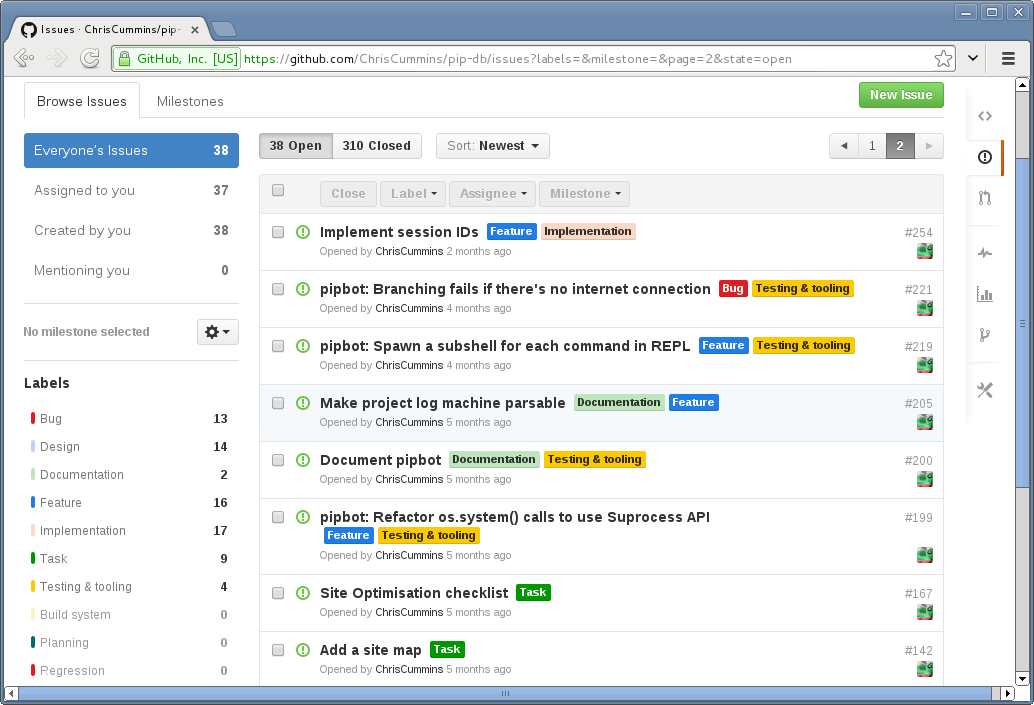
\includegraphics[width=\textwidth]{assets/github-issues}
\caption[GitHub project open issues]
        {GitHub project open issues.}
\label{fig:github-issues}
\end{figure}


% TODO: Milestones


%%%%%%%%%%%%%%%%%%%%%%%%%%%%%%%
%% Figure: github-milestones %%
%%%%%%%%%%%%%%%%%%%%%%%%%%%%%%%
\begin{figure}[H]
\centering
    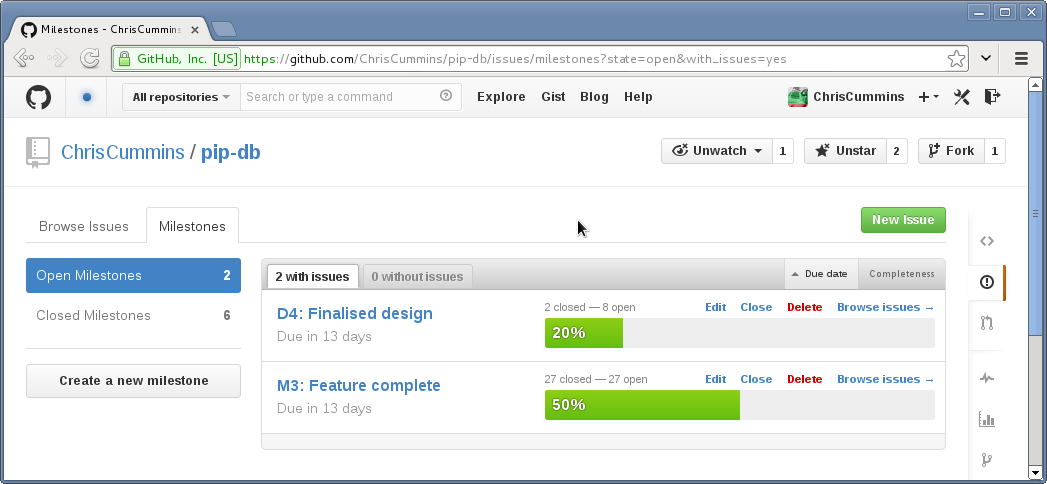
\includegraphics[width=\textwidth]{assets/github-milestones}
\caption[GitHub project open milestones]
        {GitHub project open milestones.}
\label{fig:github-milestones}
\end{figure}


\section{Design process}


\subsection{User-centred design}

% Existing systems

\cite{lu2011pubmed, hearst2007biotext}

% CRITIQUE of Darren's systems

% Usability research

\cite{bolchini2009better, pavelin2012bioinformatics}


\subsection{Low fidelity prototyping}

% TODO: Low-fi
\cite{egger2000lofi}

% TODO: Balsamiq


\subsection{High fidelity prototyping}

% TODO: Rapid prototyping using PHP + CSS + HTML + JS

% TODO: Both DESIGN and TECHNICAL prototype
